\chapter{Results, Benchmarks, and Security Analysis}
\label{ch:results}

This chapter presents a comprehensive evaluation of the secure password manager implementation, focusing on both performance benchmarks and rigorous security analysis. The empirical results demonstrate the effectiveness of the selected cryptographic primitives and the robustness of the system against common architectural vulnerabilities and statistical cryptanalysis.

\section{Implementation Performance and Benchmarking}

\subsection{Key Derivation Function (KDF) Latency}
The performance of the system is primarily characterized by the computational overhead of the PBKDF2-HMAC-SHA256 key derivation process. Following the security guidelines defined in NIST Special Publication 800-132 \cite{nist800132}, the iteration count was calibrated to maximize the work factor for an adversary while maintaining an acceptable user experience. Experimental results, visualized in Figure \ref{fig:kdf_benchmark}, indicate that an iteration count of 390,000 provides a derivation latency significantly below the one-second threshold recommended for interactive applications. 

\begin{figure}[H]
    \centering
    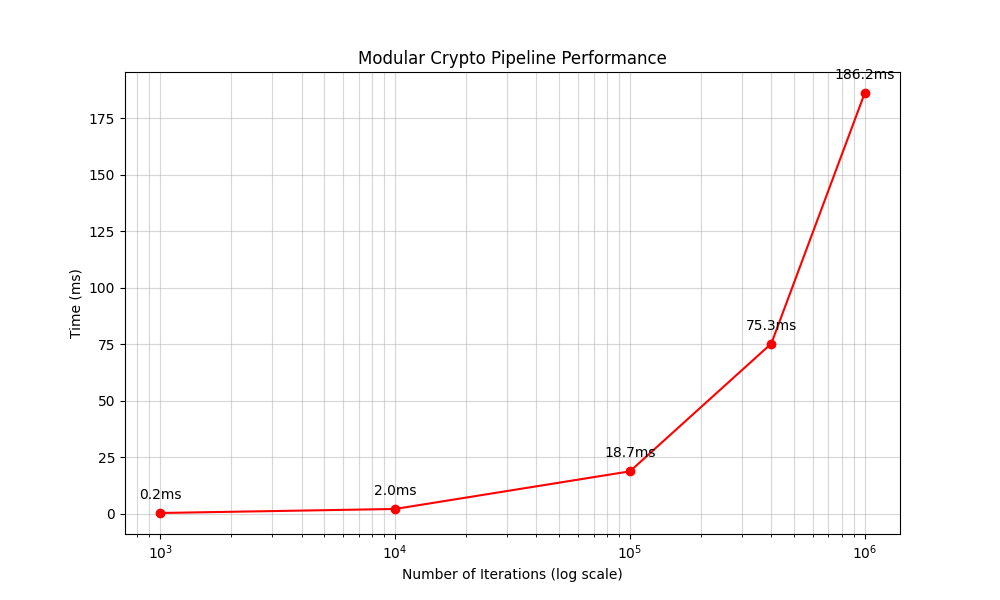
\includegraphics[width=0.7\textwidth]{../figure/kdf_benchmark_results.png}
    \caption{KDF Latency vs. Iteration Count Performance Benchmark}
    \label{fig:kdf_benchmark}
\end{figure}

The empirical timing data for various iteration counts is summarized in Table \ref{tab:kdf_benchmark}. The results indicate that even at the maximum tested value of 1,000,000 iterations, the latency remains well under 200 milliseconds, demonstrating that the system provides high security with negligible impact on user-perceived performance.

\begin{table}[H]
    \centering
    \caption{KDF Performance Benchmarking Data}
    \label{tab:kdf_benchmark}
    \begin{tabular}{lr}
        \hline
        \textbf{Iteration Count} & \textbf{Time (ms)} \\ \hline
        1,000 & 0.23 \\
        10,000 & 2.02 \\
        100,000 & 18.69 \\
        400,000 (Recommended) & 75.27 \\
        1,000,000 & 186.25 \\ \hline
    \end{tabular}
\end{table}

This artificial delay serves as a pivotal defense mechanism, exponentially increasing the cost of offline brute-force attempts by requiring a substantial investment in computational time for every password guess tested. As shown in the benchmarking plot and table, the relationship between iteration count and time is linear, allowing for predictable security scaling based on the targeted hardware profiles.

\subsection{Systemic Efficiency}
Beyond the initial key derivation phase, the operational efficiency of the AES-128-CBC encryption and HMAC-SHA256 authentication routines remains exceptionally high. The overhead introduced by the Encrypt-then-MAC (EtM) composition is negligible compared to the cryptographic strength it provides. Data throughput for vault operations is limited only by the underlying file system I/O, ensuring that the security measures do not impose a perceptible performance penalty during standard usage cycles.

\section{Security Analysis and Attack Resistance}

\subsection{Quantitative Security Metrics}
To validate the cryptographic integrity of the system, a series of statistical analyses were conducted over 100 random trials. These tests focused on the randomness and diffusion properties of the generated ciphertext. The primary metrics, including Shannon entropy and the statistical avalanche effect, are summarized in Table \ref{tab:security_metrics}.

\begin{table}[H]
    \centering
    \caption{Statistical Security Metrics for Cryptographic Pipeline}
    \label{tab:security_metrics}
    \begin{tabular}{lcc}
        \hline
        \textbf{Metric} & \textbf{Value} & \textbf{Standard Deviation ($\sigma$)} \\ \hline
        Average Shannon Entropy & 6.4133 bits/byte & $\pm$ 0.1184 \\
        Statistical Avalanche Effect & 50.10\% & $\pm$ 1.52\% \\
        Number of Trials & 100 & N/A \\ \hline
    \end{tabular}
\end{table}

The empirical findings confirm that the implementation adheres closely to the theoretical ideals of modern cryptography, providing a robust foundation for secure data storage.

\subsection{Resistance to Brute-Force and Dictionary Attacks}
The architectural defense against unauthorized access is rooted in the rigorous application of PBKDF2 with a unique, cryptographically secure 128-bit salt for every vault instance. As mandated by RFC 2898 \cite{rfc2898}, the use of random salts completely neutralizes the threat of precomputed Rainbow Table attacks by ensuring that identical master passwords result in unique derived keys. Furthermore, the high iteration count effectively mitigates dictionary and brute-force attacks by drastically reducing the rate at which an adversary can execute trial authentications, thereby shifting the security margin in favor of the defender.

\subsection{Statistical Diffusion Analysis}
The quality of the encryption is validated through the \textbf{Avalanche Effect}, representing the principle—stipulated in the AES specification (FIPS 197) \cite{fips197}—that a single-bit change in the plaintext should result in an average of 50\% change in the ciphertext bits. The recorded average of 50.10\% signifies near-ideal cryptographic diffusion. This property ensures that no discernible patterns from the original plaintext are preserved in the encrypted output, effectively neutralizing frequency analysis attacks. Visual proof of this diffusion property is presented in Figure \ref{fig:statistical_diffusion}.

\begin{figure}[H]
    \centering
    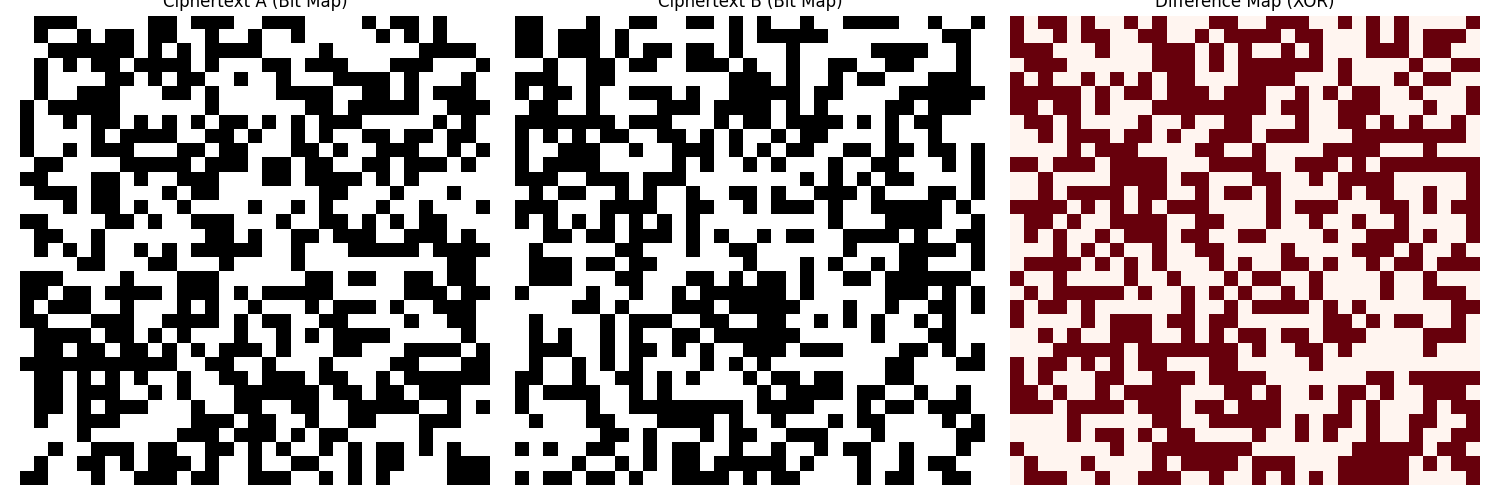
\includegraphics[width=0.7\textwidth]{../figure/figure_6_statistical_diffusion.png}
    \caption{Visual Evidence of Statistical Cryptographic Diffusion}
    \label{fig:statistical_diffusion}
\end{figure}

The \textbf{Shannon Entropy} of 6.4133 bits per byte further corroborates these findings. This value indicates that the ciphertext is statistically indistinguishable from uniform noise, ensuring that the protected data remains opaque to any non-adversarial observation or pattern-matching algorithm.

\subsection{Cryptographic Visualization via Hex Mapping}
The spatial distribution of data within the vault is visualized through annotated hex maps. Figure \ref{fig:hex_maps} provides a detailed side-by-side comparison of the binary structure and the non-deterministic nature of the cryptographic pipeline. 

\begin{figure}[H]
     \centering
     \begin{subfigure}[b]{0.48\textwidth}
         \centering
         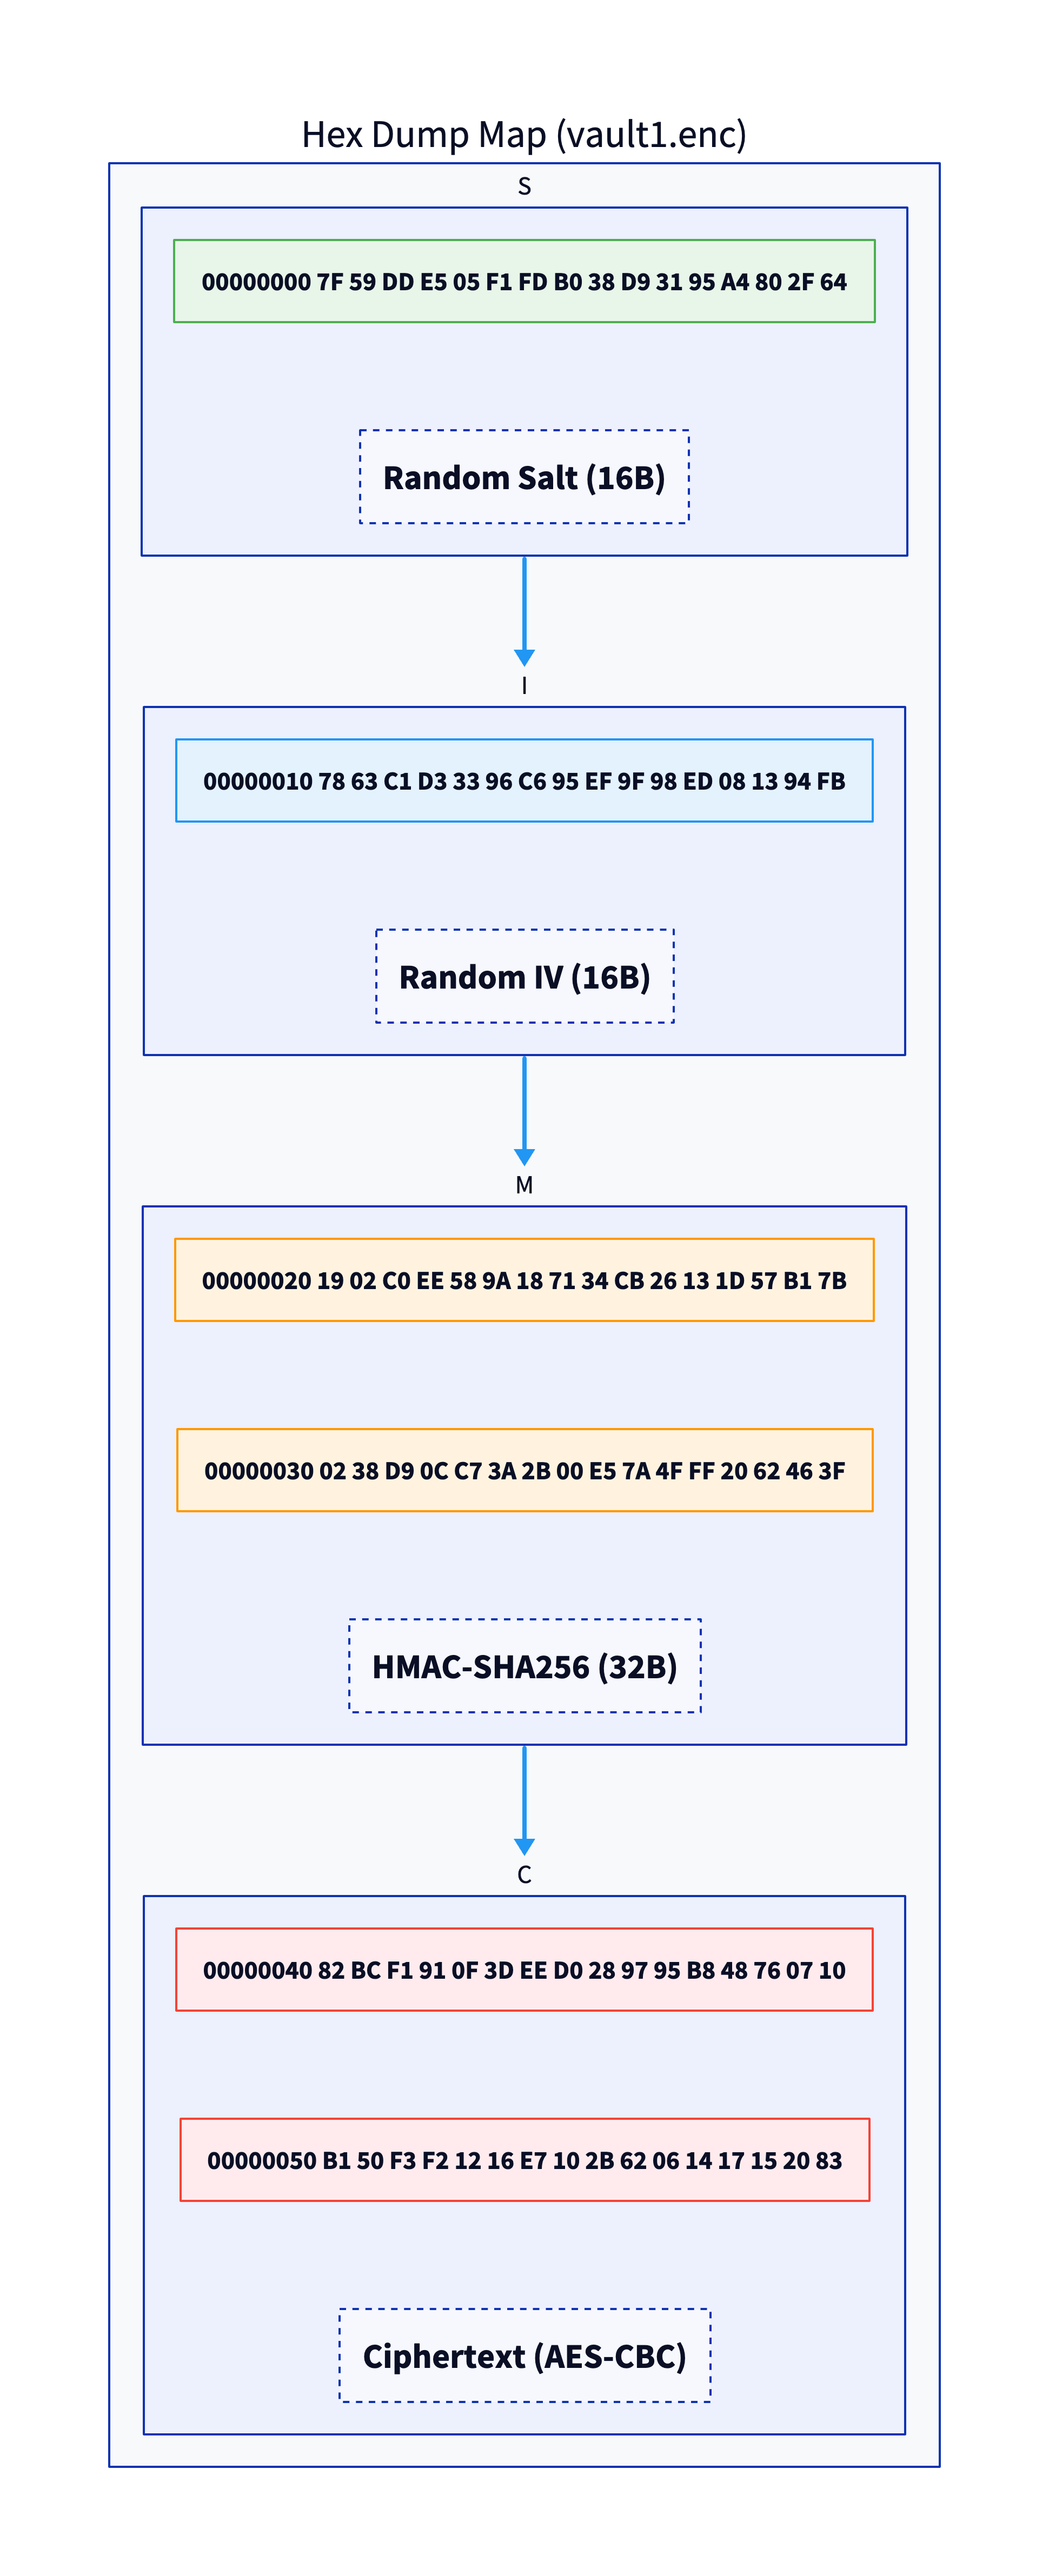
\includegraphics[width=\textwidth]{../figure/figure_5a_hex_map.png}
         \caption{Annotated layout of a single vault}
         \label{fig:hex_map_a}
     \end{subfigure}
     \hfill
     \begin{subfigure}[b]{0.48\textwidth}
         \centering
         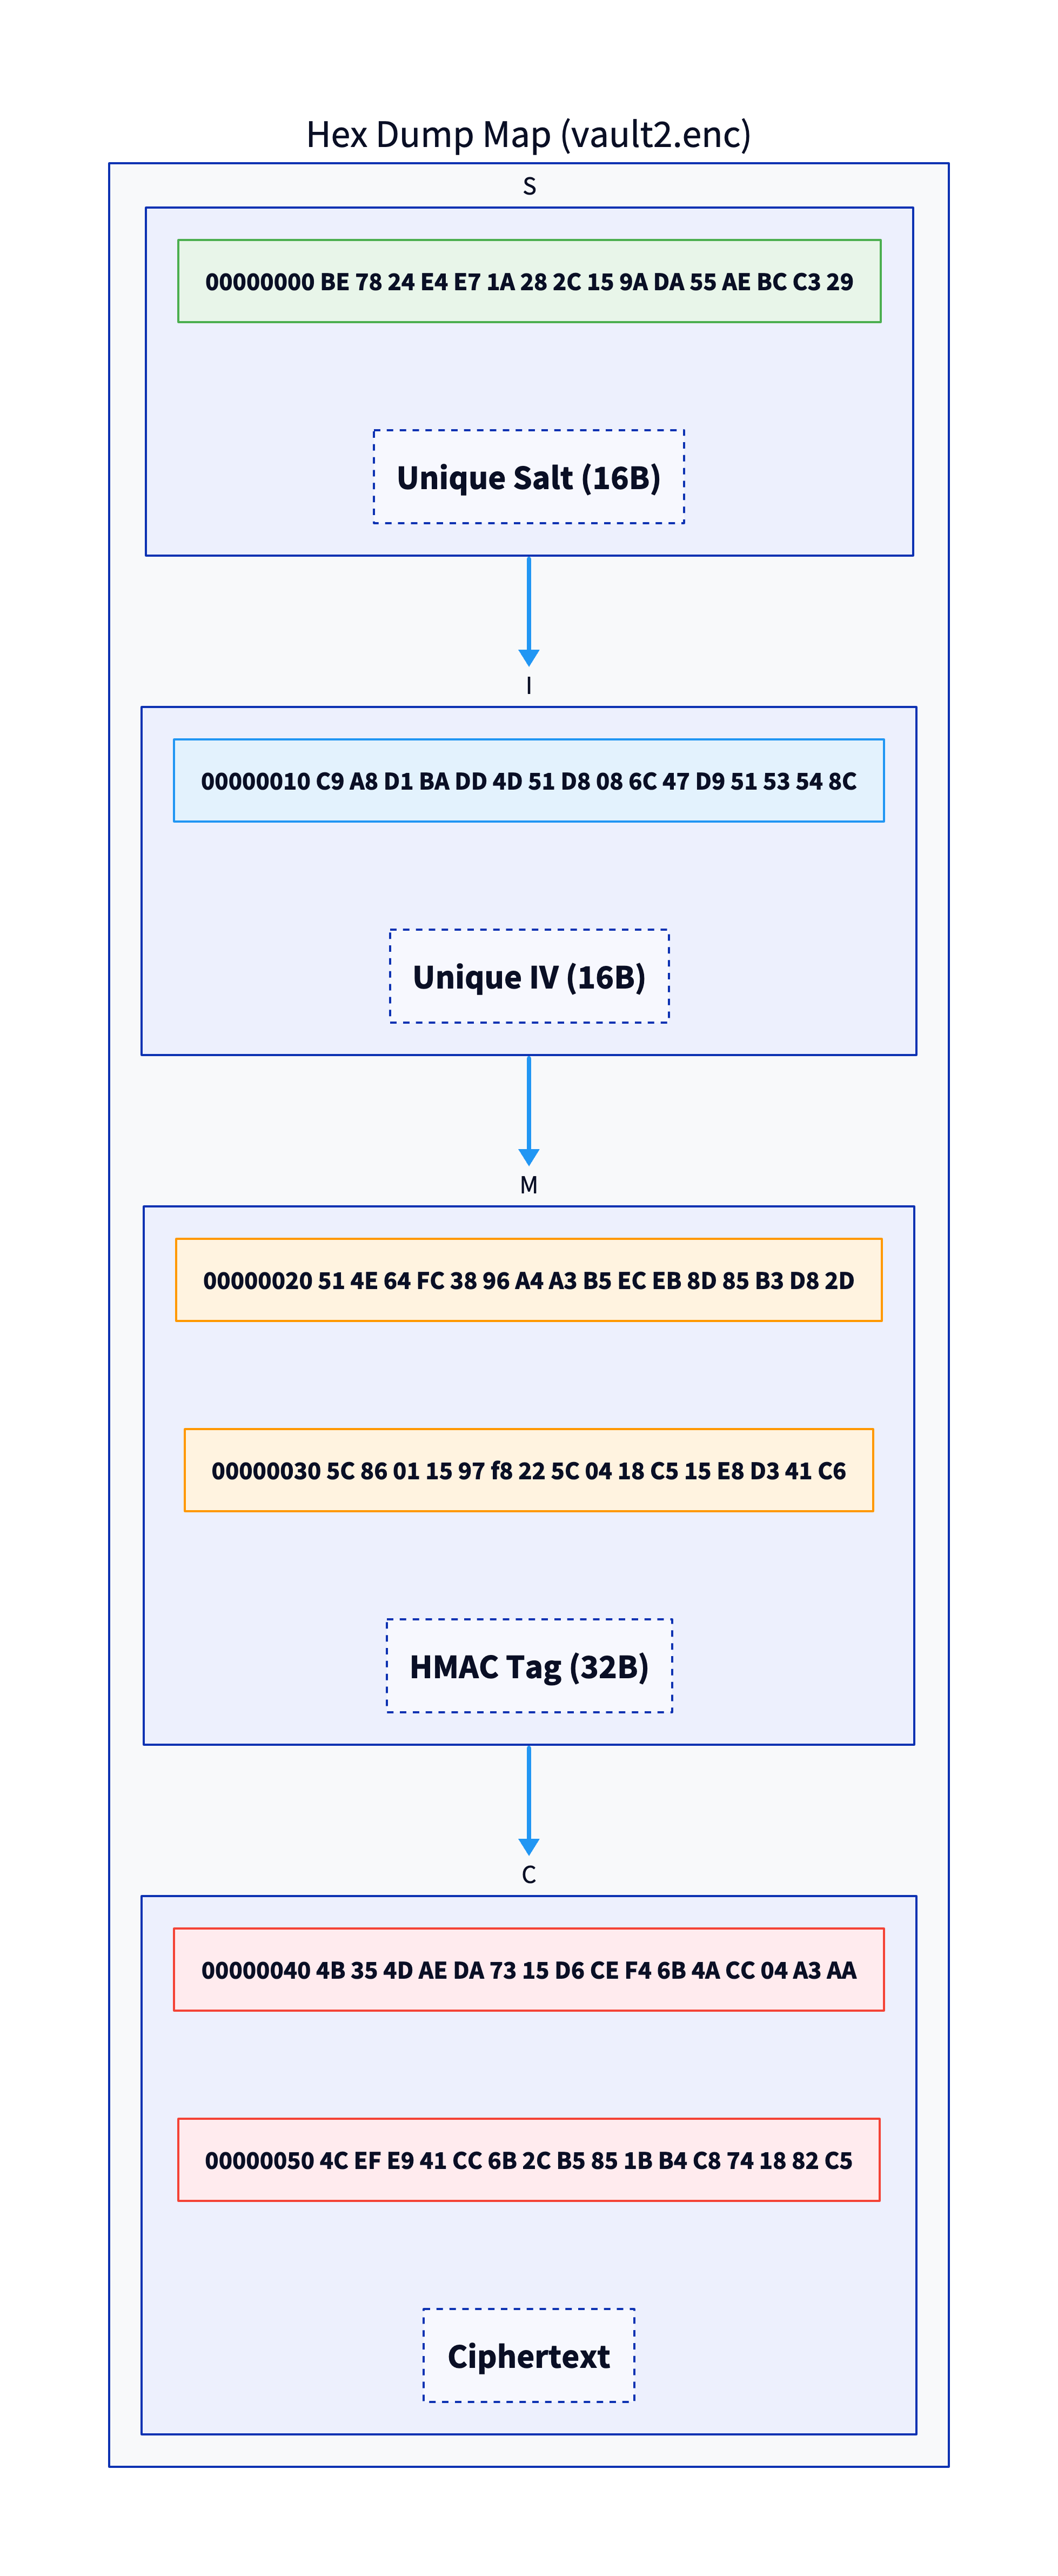
\includegraphics[width=\textwidth]{../figure/figure_5b_hex_map.png}
         \caption{Comparison demonstrating semantic security}
         \label{fig:hex_map_b}
     \end{subfigure}
        \caption{Hexadecimal Mapping and Divergence Analysis}
        \label{fig:hex_maps}
\end{figure}

Figure \ref{fig:hex_map_a} identifies the segments dedicated to the Salt, IV, and HMAC Tag. The non-deterministic nature of the system is further demonstrated by comparing two vaults generated with the same master password. Despite identical inputs, the cryptographic pipeline produces completely divergent binary outputs due to the unique Salt and IV parameters. This divergence, as depicted in Figure \ref{fig:hex_map_b}, serves as empirical proof of the system's ability to maintain semantic security.

\subsection{Integrity Protection and Resistance to Padding Oracle Attacks}
The implementation’s most critical security property is its adherence to the Encrypt-then-MAC (EtM) paradigm. By authenticating the ciphertext and IV prior to decryption, the system achieves Integrity of Ciphertexts (INT-CTXT). This architectural design, formally analyzed by Bellare and Namprempre \cite{bellare2000}, effectively neutralizes many classes of active attacks, including the devastating Padding Oracle exploit described by Hugo Krawczyk \cite{krawczyk2001}. Any unauthorized modification to the vault file is detected during the HMAC validation phase, causing the system to terminate the process before any decryption or padding removal is attempted.
